\documentclass[11pt,a4paper]{article}
%%%%%%%%%%%%%%%%%%%%%%%%% Credit %%%%%%%%%%%%%%%%%%%%%%%%

% template ini dibuat oleh martin.manullang@if.itera.ac.id untuk dipergunakan oleh seluruh sivitas akademik itera.

%%%%%%%%%%%%%%%%%%%%%%%%% PACKAGE starts HERE %%%%%%%%%%%%%%%%%%%%%%%%
\usepackage{graphicx}
\usepackage{caption}
\usepackage{microtype}
\captionsetup[table]{name=Tabel}
\captionsetup[figure]{name=Gambar}
\usepackage{tabulary}
\usepackage{minted}
% \usepackage{amsmath}
\usepackage{fancyhdr}
% \usepackage{amssymb}
% \usepackage{amsthm}
\usepackage{placeins}
% \usepackage{amsfonts}
\usepackage{graphicx}
\usepackage[all]{xy}
\usepackage{tikz}
\usepackage{verbatim}
\usepackage[left=2cm,right=2cm,top=3cm,bottom=2.5cm]{geometry}
\usepackage{hyperref}
\hypersetup{
    colorlinks,
    linkcolor={red!50!black},
    citecolor={blue!50!black},
    urlcolor={blue!80!black}
}
\usepackage{caption}
\usepackage{subcaption}
\usepackage{multirow}
\usepackage{psfrag}
\usepackage[T1]{fontenc}
\usepackage[scaled]{beramono}
% Enable inserting code into the document
\usepackage{listings}
\usepackage{xcolor} 
% custom color & style for listing
\definecolor{codegreen}{rgb}{0,0.6,0}
\definecolor{codegray}{rgb}{0.5,0.5,0.5}
\definecolor{codepurple}{rgb}{0.58,0,0.82}
\definecolor{backcolour}{rgb}{0.95,0.95,0.92}
\definecolor{LightGray}{gray}{0.9}
\lstdefinestyle{mystyle}{
	backgroundcolor=\color{backcolour},   
	commentstyle=\color{green},
	keywordstyle=\color{codegreen},
	numberstyle=\tiny\color{codegray},
	stringstyle=\color{codepurple},
	basicstyle=\ttfamily\footnotesize,
	breakatwhitespace=false,         
	breaklines=true,                 
	captionpos=b,                    
	keepspaces=true,                 
	numbers=left,                    
	numbersep=5pt,                  
	showspaces=false,                
	showstringspaces=false,
	showtabs=false,                  
	tabsize=2
}
\lstset{style=mystyle}
\renewcommand{\lstlistingname}{Kode}
%%%%%%%%%%%%%%%%%%%%%%%%% PACKAGE ends HERE %%%%%%%%%%%%%%%%%%%%%%%%


%%%%%%%%%%%%%%%%%%%%%%%%% Data Diri %%%%%%%%%%%%%%%%%%%%%%%%
\newcommand{\student}{\textbf{Irwanto Yezekiel Sihotang (120140227)}}
\newcommand{\course}{\textbf{Sistem Operasi RA (IF2223)}}
\newcommand{\assignment}{\textbf{2}}

%%%%%%%%%%%%%%%%%%% using theorem style %%%%%%%%%%%%%%%%%%%%
\newtheorem{thm}{Theorem}
\newtheorem{lem}[thm]{Lemma}
\newtheorem{defn}[thm]{Definition}
\newtheorem{exa}[thm]{Example}
\newtheorem{rem}[thm]{Remark}
\newtheorem{coro}[thm]{Corollary}
\newtheorem{quest}{Question}[section]
%%%%%%%%%%%%%%%%%%%%%%%%%%%%%%%%%%%%%%%%
\usepackage{lipsum}%% a garbage package you don't need except to create examples.
\usepackage{fancyhdr}
\pagestyle{fancy}
\lhead{Irwanto Yezekiel Sihotang (120140227)}
\rhead{ \thepage}
\cfoot{\textbf{HandsOn 2 : Synchronisation and Deadlock}}
\renewcommand{\headrulewidth}{0.4pt}
\renewcommand{\footrulewidth}{0.4pt}

%%%%%%%%%%%%%%  Shortcut for usual set of numbers  %%%%%%%%%%%

\newcommand{\N}{\mathbb{N}}
\newcommand{\Z}{\mathbb{Z}}
\newcommand{\Q}{\mathbb{Q}}
\newcommand{\R}{\mathbb{R}}
\newcommand{\C}{\mathbb{C}}
\setlength\headheight{14pt}

%%%%%%%%%%%%%%%%%%%%%%%%%%%%%%%%%%%%%%%%%%%%%%%%%%%%%%%555
\begin{document}
\thispagestyle{empty}
\begin{center}
	
\includegraphics[scale = 0.15]{Figure/ifitera-header.png}
	\vspace{0.1cm}
\end{center}
\noindent
\rule{17cm}{0.2cm}\\[0.3cm]
Nama: \student \hfill Tugas Ke: \assignment\\[0.1cm]
Mata Kuliah: \course \hfill Tanggal: 11 April 2022\\
\rule{17cm}{0.05cm}
\vspace{0.1cm}



%%%%%%%%%%%%%%%%%%%%%%%%%%%%%%%%%%%%%%%%%%%%% BODY DOCUMENT %%%%%%%%%%%%%%%%%%%%%%%%%%%%%%%%%%%%%%%%%%%%%
\section{Tujuan Hands On 2}
    tujuan dari tugas Hands On dua ini adalah Agar memahami sistem sinkronisasi dan permasalahan yang ada serta Memahami solusi dalam menangani critical section. adapun hal yang harus dipahami dalam tugas Hands On dua ini adalah implementasi dari join menggunakan semaphores, Binary Semaphores, Producer Consumer, Reader / Writer Locks dan Dining Philosophers. 

\section{Fork/Join}

\subsection{Source Code}
\begin{lstlisting}[language=Python, code fork join,label={labelkode}]
#include <stdio.h>
#include <stdlib.h>
#include <pthread.h>
#include <unistd.h>

#include "common.h"
#include "common_threads.h"

#ifdef linux
#include <semaphore.h>
#elif _APPLE_
#include "zemaphore.h"
#endif

sem_t s;

void *child(void *arg) {
    sleep(2);
    printf("child\n");
    Sem_post(&s); // signal here: child is done
    return NULL;
}

int main(int argc, char *argv[]) {
    Sem_init(&s, 0); 
    printf("parent: begin\n");
    pthread_t c;
    Pthread_create(&c, NULL, child, NULL);
    Sem_wait(&s); // wait here for child
    printf("parent: end\n");
    return 0;
}
    \end{lstlisting}
    
\subsection{Output}
\begin{figure}[h]
    \centering
    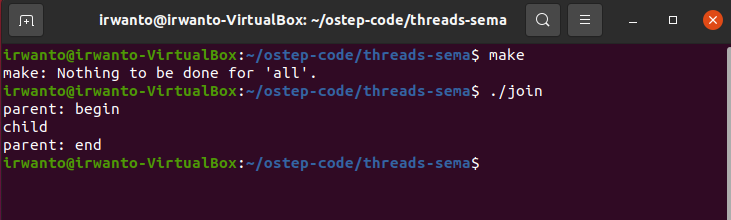
\includegraphics[width=0.8\textwidth]{Figure/join.png}
    \caption{Fork/Join}
    \label{fig:my_label}
\end{figure}

\subsection{Penjelasan Fork/Join}
semaphore adalah suatu struktur data komputer yang berguna untuk sinkronisasi proses dan berfungsi memerintahkan program agar menjalankan proses. contohnya adalah \textit{thread} menunggu \textit{list} sehingga \textit{list} menjadi berisi atau tidak kosong. Dalam kondisi tersebut, semaphore akan didefinisikan dan dimulai ke 0 oleh Sem init. Tujuan dari proses ini adalah semaphore akan dibagikan di antara \textit{thread} dalam proses yang sama. Kemudian ketika pembuatan \textit{thread} selesai, akan terus memanggil fungsi child semaphore yang akan memberi sinyal bahwa proses child selesai dan dimulai kembali. Ketika child Setelah selesai, semaphore akan melanjutkan dan menampilkan "parent : end".

\section{Binary Semaphores}
\subsection{Source Code}
\begin{lstlisting}[language=Python, caption=Code Binary semaphores,label={labelkode}]
#include <stdio.h>
#include <stdlib.h>
#include <pthread.h>
#include <unistd.h>

#include "common.h"
#include "common_threads.h"

#ifdef linux
#include <semaphore.h>
#elif __APPLE__
#include "zemaphore.h"
#endif

sem_t mutex;
volatile int counter = 0;

void *child(void *arg) {
    int i;
    for (i = 0; i < 10000000; i++) {
	Sem_wait(&mutex);
	counter++;
	Sem_post(&mutex);
    }
    return NULL;
}

int main(int argc, char *argv[]) {
    Sem_init(&mutex, 1); 
    pthread_t c1, c2;
    Pthread_create(&c1, NULL, child, NULL);
    Pthread_create(&c2, NULL, child, NULL);
    Pthread_join(c1, NULL);
    Pthread_join(c2, NULL);
    printf("result: %d (should be 20000000)\n", counter);
    return 0;
}
    \end{lstlisting}

\subsection{Output}
\begin{figure}[h]
    \centering
    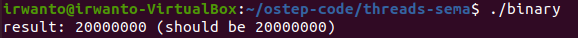
\includegraphics[width=0.8\textwidth]{Figure/binary1.png}
    \caption{Binary Semaphores}
    \label{fig:my_label}
\end{figure}

\subsection{Penjelasan Binary Semaphores}
Pada kode di atas terdapat variabel \textit{sem t mutex} atau bisa disebut \textit{mutual exclusion} berperan dalam mengelola penggunaan \textit{resource}. Mutex ada untuk mencegah kondisi balapan. Pertama kita set dan inisialisasi semaphore mutex dengan nilai 1, Selanjutnya, sebuah \textit{thread} dibuat dengan inisial c1 dan c2, yang berguna dalam menjalankan fungsi child. Kemudian i akan menginisialisasi dalam \textit{loop} sampai nilai i kurang dari 10000000 untuk dieksekusi \textit{sem wait} dan pada saat itu \textit{value} akan berkurang dan \textit{critical section} akan dimulai, akan ada tambahan nilai \textit{counter} yang kemudian semaphore akan memproses panggilan untuk menaikkan nilai semaphore sebagai sinyal bahwa \textit{critical section} sudah selesai. Kemudian program akan mengulangi prosesnya sampai kondisi terpenuhi, \textit{thread} c2 akan terus menjalankan fungsi \textit{child}. Ketika selesai, akan memulai \textit{return} fungsi \textit{main} yang akan menampilkan hasil penghitung dieksekusi menampilkan output dalam nilai 20000000.

\section{Producer Consumer}
\subsection{Source Code}
\begin{lstlisting}[language=Python, caption=source code Producer Consumer,label={labelkode}]
#include <stdio.h>
#include <unistd.h>
#include <assert.h>
#include <pthread.h>
#include <stdlib.h>

#include "common.h"
#include "common_threads.h"

#ifdef linux
#include <semaphore.h>
#elif __APPLE__
#include "zemaphore.h"
#endif

int max;
int loops;
int *buffer;

int use  = 0;
int fill = 0;

sem_t empty;
sem_t full;
sem_t mutex;

#define CMAX (10)
int consumers = 1;

void do_fill(int value) {
    buffer[fill] = value;
    fill++;
    if (fill == max)
	fill = 0;
}

int do_get() {
    int tmp = buffer[use];
    use++;
    if (use == max)
	use = 0;
    return tmp;
}

void *producer(void *arg) {
    int i;
    for (i = 0; i < loops; i++) {
	Sem_wait(&empty);
	Sem_wait(&mutex);
	do_fill(i);
	Sem_post(&mutex);
	Sem_post(&full);
    }

    // end case
    for (i = 0; i < consumers; i++) {
	Sem_wait(&empty);
	Sem_wait(&mutex);
	do_fill(-1);
	Sem_post(&mutex);
	Sem_post(&full);
    }

    return NULL;
}
                                                                               
void *consumer(void *arg) {
    int tmp = 0;
    while (tmp != -1) {
	Sem_wait(&full);
	Sem_wait(&mutex);
	tmp = do_get();
	Sem_post(&mutex);
	Sem_post(&empty);
	printf("%lld %d\n", (long long int) arg, tmp);
    }
    return NULL;
}

int main(int argc, char *argv[]) {
    if (argc != 4) {
	fprintf(stderr, "usage: %s <buffersize> <loops> <consumers>\n", argv[0]);
	exit(1);
    }
    max   = atoi(argv[1]);
    loops = atoi(argv[2]);
    consumers = atoi(argv[3]);
    assert(consumers <= CMAX);

    buffer = (int *) malloc(max * sizeof(int));
    assert(buffer != NULL);
    int i;
    for (i = 0; i < max; i++) {
	buffer[i] = 0;
    }

    Sem_init(&empty, max); // max are empty 
    Sem_init(&full, 0);    // 0 are full
    Sem_init(&mutex, 1);   // mutex

    pthread_t pid, cid[CMAX];
    Pthread_create(&pid, NULL, producer, NULL); 
    for (i = 0; i < consumers; i++) {
	Pthread_create(&cid[i], NULL, consumer, (void *) (long long int) i); 
    }
    Pthread_join(pid, NULL); 
    for (i = 0; i < consumers; i++) {
	Pthread_join(cid[i], NULL); 
    }
    return 0;
}
    \end{lstlisting}

\subsection{Output}
\begin{figure}[h]
    \centering
    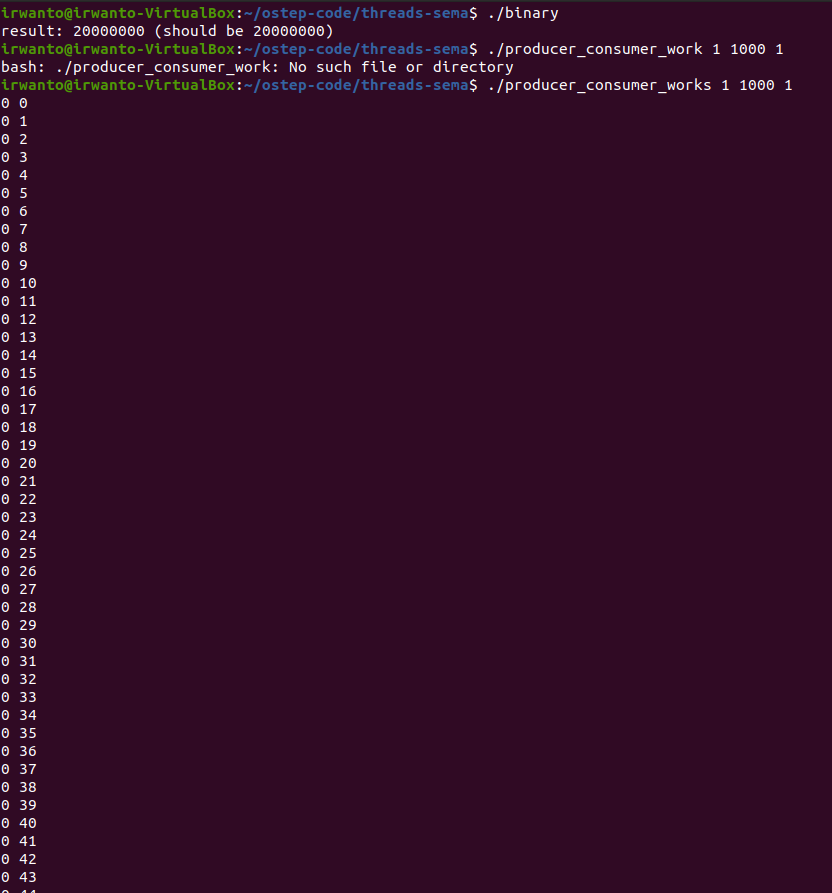
\includegraphics[width=0.8\textwidth]{Figure/producer consumer.png}
    \caption{Producer Consumer}
    \label{fig:my_label}
\end{figure}

\subsection{Penjelasan Producer Consumer}
Implementasi \textit{producer/konsumer} disebut \textit{bounded buffer}. Isi dari program ini adalah untuk memanggil, mengurangi, menghalangi consumer dan berharap \textit{thread} lainnya dapat memanggil \textit{Sem post} ketika sudah penuh.Kemudian program akan memulai fungsi prosedur yang berguna untuk memanggil \textit{sem wait}(\textit{emty}) dan \textit{sem post} (mutex). \textit{Producer} akan diisi dengan fungsi \textit{do fill} pada input pertama \textit{buffer} setelah emty dikurangi menjadi nilai 0. Kemudian Producer akan terus berjalan sampai panggilan \textit{sem post}(mutex) dan \textit{sem post}(full) yang akan merubah nilai total dari -1 menjadi 0. Jadi Konsumen akan mengulang dan memblok dengan \textit{value semaphore} kosong.

\section{Reader / Writer Locks}
\subsection{Source Code}
\begin{lstlisting}[language=Python, caption=source code Reader / writer locks,label={labelkode}]
#include <stdio.h>
#include <unistd.h>
#include <assert.h>
#include <pthread.h>
#include <stdlib.h>

#include "common.h"
#include "common_threads.h"

#ifdef linux
#include <semaphore.h>
#elif __APPLE__
#include "zemaphore.h"
#endif

int max;
int loops;
int *buffer;

int use  = 0;
int fill = 0;

sem_t empty;
sem_t full;
sem_t mutex;

#define CMAX (10)
int consumers = 1;

void do_fill(int value) {
    buffer[fill] = value;
    fill++;
    if (fill == max)
	fill = 0;
}

int do_get() {
    int tmp = buffer[use];
    use++;
    if (use == max)
	use = 0;
    return tmp;
}

void *producer(void *arg) {
    int i;
    for (i = 0; i < loops; i++) {
	Sem_wait(&empty);
	Sem_wait(&mutex);
	do_fill(i);
	Sem_post(&mutex);
	Sem_post(&full);
    }

    // end case
    for (i = 0; i < consumers; i++) {
	Sem_wait(&empty);
	Sem_wait(&mutex);
	do_fill(-1);
	Sem_post(&mutex);
	Sem_post(&full);
    }

    return NULL;
}
                                                                               
void *consumer(void *arg) {
    int tmp = 0;
    while (tmp != -1) {
	Sem_wait(&full);
	Sem_wait(&mutex);
	tmp = do_get();
	Sem_post(&mutex);
	Sem_post(&empty);
	printf("%lld %d\n", (long long int) arg, tmp);
    }
    return NULL;
}

int main(int argc, char *argv[]) {
    if (argc != 4) {
	fprintf(stderr, "usage: %s <buffersize> <loops> <consumers>\n", argv[0]);
	exit(1);
    }
    max   = atoi(argv[1]);
    loops = atoi(argv[2]);
    consumers = atoi(argv[3]);
    assert(consumers <= CMAX);

    buffer = (int *) malloc(max * sizeof(int));
    assert(buffer != NULL);
    int i;
    for (i = 0; i < max; i++) {
	buffer[i] = 0;
    }

    Sem_init(&empty, max); // max are empty 
    Sem_init(&full, 0);    // 0 are full
    Sem_init(&mutex, 1);   // mutex

    pthread_t pid, cid[CMAX];
    Pthread_create(&pid, NULL, producer, NULL); 
    for (i = 0; i < consumers; i++) {
	Pthread_create(&cid[i], NULL, consumer, (void *) (long long int) i); 
    }
    Pthread_join(pid, NULL); 
    for (i = 0; i < consumers; i++) {
	Pthread_join(cid[i], NULL); 
    }
    return 0;
}
    \end{lstlisting}

\subsection{Output}
\begin{figure}[h]
    \centering
    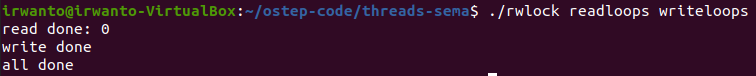
\includegraphics[width=0.8\textwidth]{Figure/read lock.png}
    \caption{Reader / Writer Locks}
    \label{fig:my_label}
\end{figure}

\subsection{Penjelasan Reader / Writer Locks}
Secara umum, \textit{semaphore writelock} untuk memastikan bahwa hanya satu \textit{writer} yang di \textit{lock} dan perbarui struktur data untuk menyertakan \textit{critical section}. Keadaan di mana \textit{lock} diperoleh, \textit{reader} yang pertama men-\textit{lock} dan mulai menambahkan variabel pembaca untuk melacak berapa banyak pembaca saat ini di struktur data. Perhatikan bahwa rwlock acquire readlock terjadi ketika pembaca pertama mendapatkan \textit{lock} dan menulis \textit{lock} dengan Tidak menunggu semaphore writelock dilepaskan saat memanggil Sem post.

\section{Dining Philosophers}
\subsection{Deadlock}
\subsubsection{Source Code}
\begin{lstlisting}[language=Python, caption=source code deadlock,label={labelkode}]
#include <stdio.h>
#include <stdlib.h>
#include <pthread.h>

#include "common.h"
#include "common_threads.h"

#ifdef linux
#include <semaphore.h>
#elif __APPLE__
#include "zemaphore.h"
#endif

typedef struct {
    int num_loops;
    int thread_id;
} arg_t;

sem_t forks[5];
sem_t print_lock;

void space(int s) {
    Sem_wait(&print_lock);
    int i;
    for (i = 0; i < s * 10; i++)
	printf(" ");
}

void space_end() {
    Sem_post(&print_lock);
}

int left(int p)  {
    return p;
}

int right(int p) {
    return (p + 1) % 5;
}

void get_forks(int p) {
    space(p); printf("%d: try %d\n", p, left(p)); space_end();
    Sem_wait(&forks[left(p)]);
    space(p); printf("%d: try %d\n", p, right(p)); space_end();
    Sem_wait(&forks[right(p)]);
}

void put_forks(int p) {
    Sem_post(&forks[left(p)]);
    Sem_post(&forks[right(p)]);
}

void think() {
    return;
}

void eat() {
    return;
}

void *philosopher(void *arg) {
    arg_t *args = (arg_t *) arg;

    space(args->thread_id); printf("%d: start\n", args->thread_id); space_end();

    int i;
    for (i = 0; i < args->num_loops; i++) {
	space(args->thread_id); printf("%d: think\n", args->thread_id); space_end();
	think();
	get_forks(args->thread_id);
	space(args->thread_id); printf("%d: eat\n", args->thread_id); space_end();
	eat();
	put_forks(args->thread_id);
	space(args->thread_id); printf("%d: done\n", args->thread_id); space_end();
    }
    return NULL;
}
                                                                             
int main(int argc, char *argv[]) {
    if (argc != 2) {
	fprintf(stderr, "usage: dining_philosophers <num_loops>\n");
	exit(1);
    }
    printf("dining: started\n");
    
    int i;
    for (i = 0; i < 5; i++) 
	Sem_init(&forks[i], 1);
    Sem_init(&print_lock, 1);

    pthread_t p[5];
    arg_t a[5];
    for (i = 0; i < 5; i++) {
	a[i].num_loops = atoi(argv[1]);
	a[i].thread_id = i;
	Pthread_create(&p[i], NULL, philosopher, &a[i]);
    }

    for (i = 0; i < 5; i++) 
	Pthread_join(p[i], NULL); 

    printf("dining: finished\n");
    return 0;
}
    \end{lstlisting}
\newpage
\subsubsection{Output}
\begin{figure}[h]
    \centering
    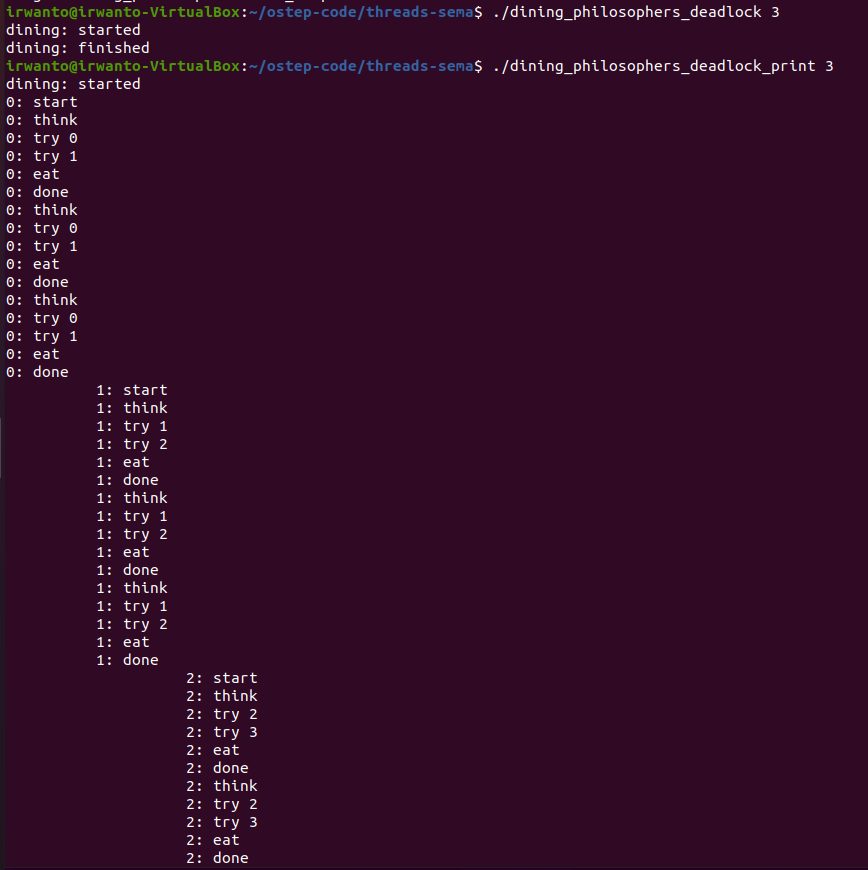
\includegraphics[width=0.7\textwidth]{Figure/5benar.png}
    \caption{Dining Philosophers deadlock}
    \label{fig:my_label}
\end{figure}

\subsubsection{Penjelasan Dining Philosophers deadlock}
Dalam pelaksanaan program \textit{Dining Philosopher Deadlock}, ada cerita menarik di baliknya. Ada masalah konkurensi yang dulu terkenal yang hanya bisa diselesaikan oleh Djikstra, masalah yang terkenal lucu dan menarik secara intelektual, yaitu masalah Philosopher's. kodisi Ketika 5 \textit{philoshoper} duduk mengelilingi meja bundar, ada sepasang \textit{philoshoper single fork} yang dimana untuk memulai makan membutuhkan sepasang \textit{fork} satu di kanan dan satu di kiri. Dengan solusi Downey, dibutuhkan beberapa fungsi pembantu yang disebut \textit{left} dan \textit{right}. Kondisi di mana \textit{philoshoper} P diminta untuk merujuk ke \textit{fork} kiri akan mulai memanggil fungsi \textit{left}, dan jika tidak, jika diminta untuk merujuk ke \textit{fork} yang benar, itu akan memanggil fungsi yang benar.  Terdapat modulo yang mana menangani satu persoalan yaitu philosopher akhir dengan P sama dengan 4 mengambil fork bagian kanan saat fork bernilai kosong.


\subsection{no Deadlock}
\subsubsection{Source Code}
\begin{lstlisting}[language=Python, caption=source code no deadlock,label={labelkode}]
#include <stdio.h>
#include <stdlib.h>
#include <pthread.h>

#include "common.h"
#include "common_threads.h"

#ifdef linux
#include <semaphore.h>
#elif __APPLE__
#include "zemaphore.h"
#endif

typedef struct {
    int num_loops;
    int thread_id;
} arg_t;

sem_t forks[5];
sem_t print_lock;

void space(int s) {
    Sem_wait(&print_lock);
    int i;
    for (i = 0; i < s * 10; i++)
	printf(" ");
}

void space_end() {
    Sem_post(&print_lock);
}

int left(int p)  {
    return p;
}

int right(int p) {
    return (p + 1) % 5;
}

void get_forks(int p) {
    if (p == 4) {
	space(p); printf("4 try %d\n", right(p)); space_end();
	Sem_wait(&forks[right(p)]);
	space(p); printf("4 try %d\n", left(p)); space_end();
	Sem_wait(&forks[left(p)]);
    } else {
	space(p); printf("try %d\n", left(p)); space_end();
	Sem_wait(&forks[left(p)]);
	space(p); printf("try %d\n", right(p)); space_end();
	Sem_wait(&forks[right(p)]);
    }
}

void put_forks(int p) {
    Sem_post(&forks[left(p)]);
    Sem_post(&forks[right(p)]);
}

void think() {
    return;
}

void eat() {
    return;
}

void *philosopher(void *arg) {
    arg_t *args = (arg_t *) arg;

    space(args->thread_id); printf("%d: start\n", args->thread_id); space_end();

    int i;
    for (i = 0; i < args->num_loops; i++) {
	space(args->thread_id); printf("%d: think\n", args->thread_id); space_end();
	think();
	get_forks(args->thread_id);
	space(args->thread_id); printf("%d: eat\n", args->thread_id); space_end();
	eat();
	put_forks(args->thread_id);
	space(args->thread_id); printf("%d: done\n", args->thread_id); space_end();
    }
    return NULL;
}
                                                                             
int main(int argc, char *argv[]) {
    if (argc != 2) {
	fprintf(stderr, "usage: dining_philosophers <num_loops>\n");
	exit(1);
    }
    printf("dining: started\n");
    
    int i;
    for (i = 0; i < 5; i++) 
	Sem_init(&forks[i], 1);
    Sem_init(&print_lock, 1);

    pthread_t p[5];
    arg_t a[5];
    for (i = 0; i < 5; i++) {
	a[i].num_loops = atoi(argv[1]);
	a[i].thread_id = i;
	Pthread_create(&p[i], NULL, philosopher, &a[i]);
    }

    for (i = 0; i < 5; i++) 
	Pthread_join(p[i], NULL); 

    printf("dining: finished\n");
    return 0;
}
    \end{lstlisting}

\newpage
\subsubsection{Output}
\begin{figure}[h]
    \centering
    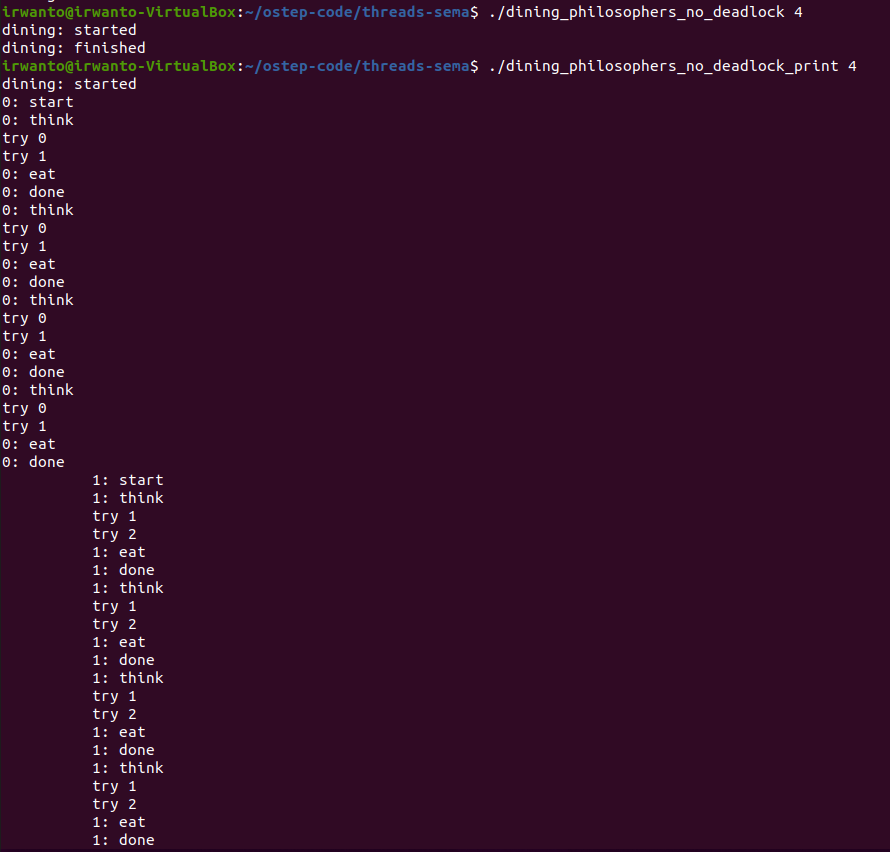
\includegraphics[width=0.7\textwidth]{Figure/5benar2.png}
    \caption{Dining Philosophers no deadlock}
    \label{fig:my_label}
\end{figure}

\subsubsection{Penjelasan Dining Philosophers no deadlock}
Pada implementasi program Dining Philosophers No Deadlock di atas menjelaskan tentang percobaan menginisialisasi setiap semaphore pada fork array sehingga memiliki nilai 1. Fakta yang menarik adalah bahwa Philosopher memiliki angka dan juga kita bisa menulis get fork dan put fork terus menerus. Kemudian, kita membutuhkan lock untuk menemukan fork di kiri dan melanjutkan di kanan. Selanjutnya, ketika kita Setelah digunakan pasti akan kita lepaskan, tapi kondisi ini tidak terjadi karena deadlock.


\section{KESIMPULAN}
tujuan dari tugas Hands On dua ini adalah Agar memahami sistem sinkronisasi dan permasalahan yangcada serta Memahami solusi dalam menangani critical section. dengan mempelajari tugas Hands On 2 ini, saya dapat memahami lebih dalam tentang materi Synchronisation and Deadlock dengan adanya pemberian kode program dari suatu programmer yang membuat programnya sesuai dengan implementasi materi tersebut serta memahami tentang adanya penggunaan Semaphores pada program yang telah dijalankan. adapun hal yang harus dipahami dalam tugas Hands On dua ini adalah implementasi dari join menggunakan semaphores, Binary Semaphores, Producer Consumer, Reader / Writer Locks dan Dining Philosophers.




newpage
\section{link GitHub}
    berikut saya lampirkan link GitHub :
\begin{itemize}
    \item \href{https://github.com/irwantoYS/Sistem-Operasi-Hands-On-2}{(Sumber: tugas Handson 2)}.
\end{itemize}

\end{document}